\section{Simultaneous measurement of fiducial cross sections for \texorpdfstring{$\Hllll$}{H to 4l} and \texorpdfstring{$\Zllll$}{Z to 4l}}

%\begin{figure}[!h!tb]
%  \begin{center}
%
%    \subfigure[$\pt(\mathrm{H})$]{
%      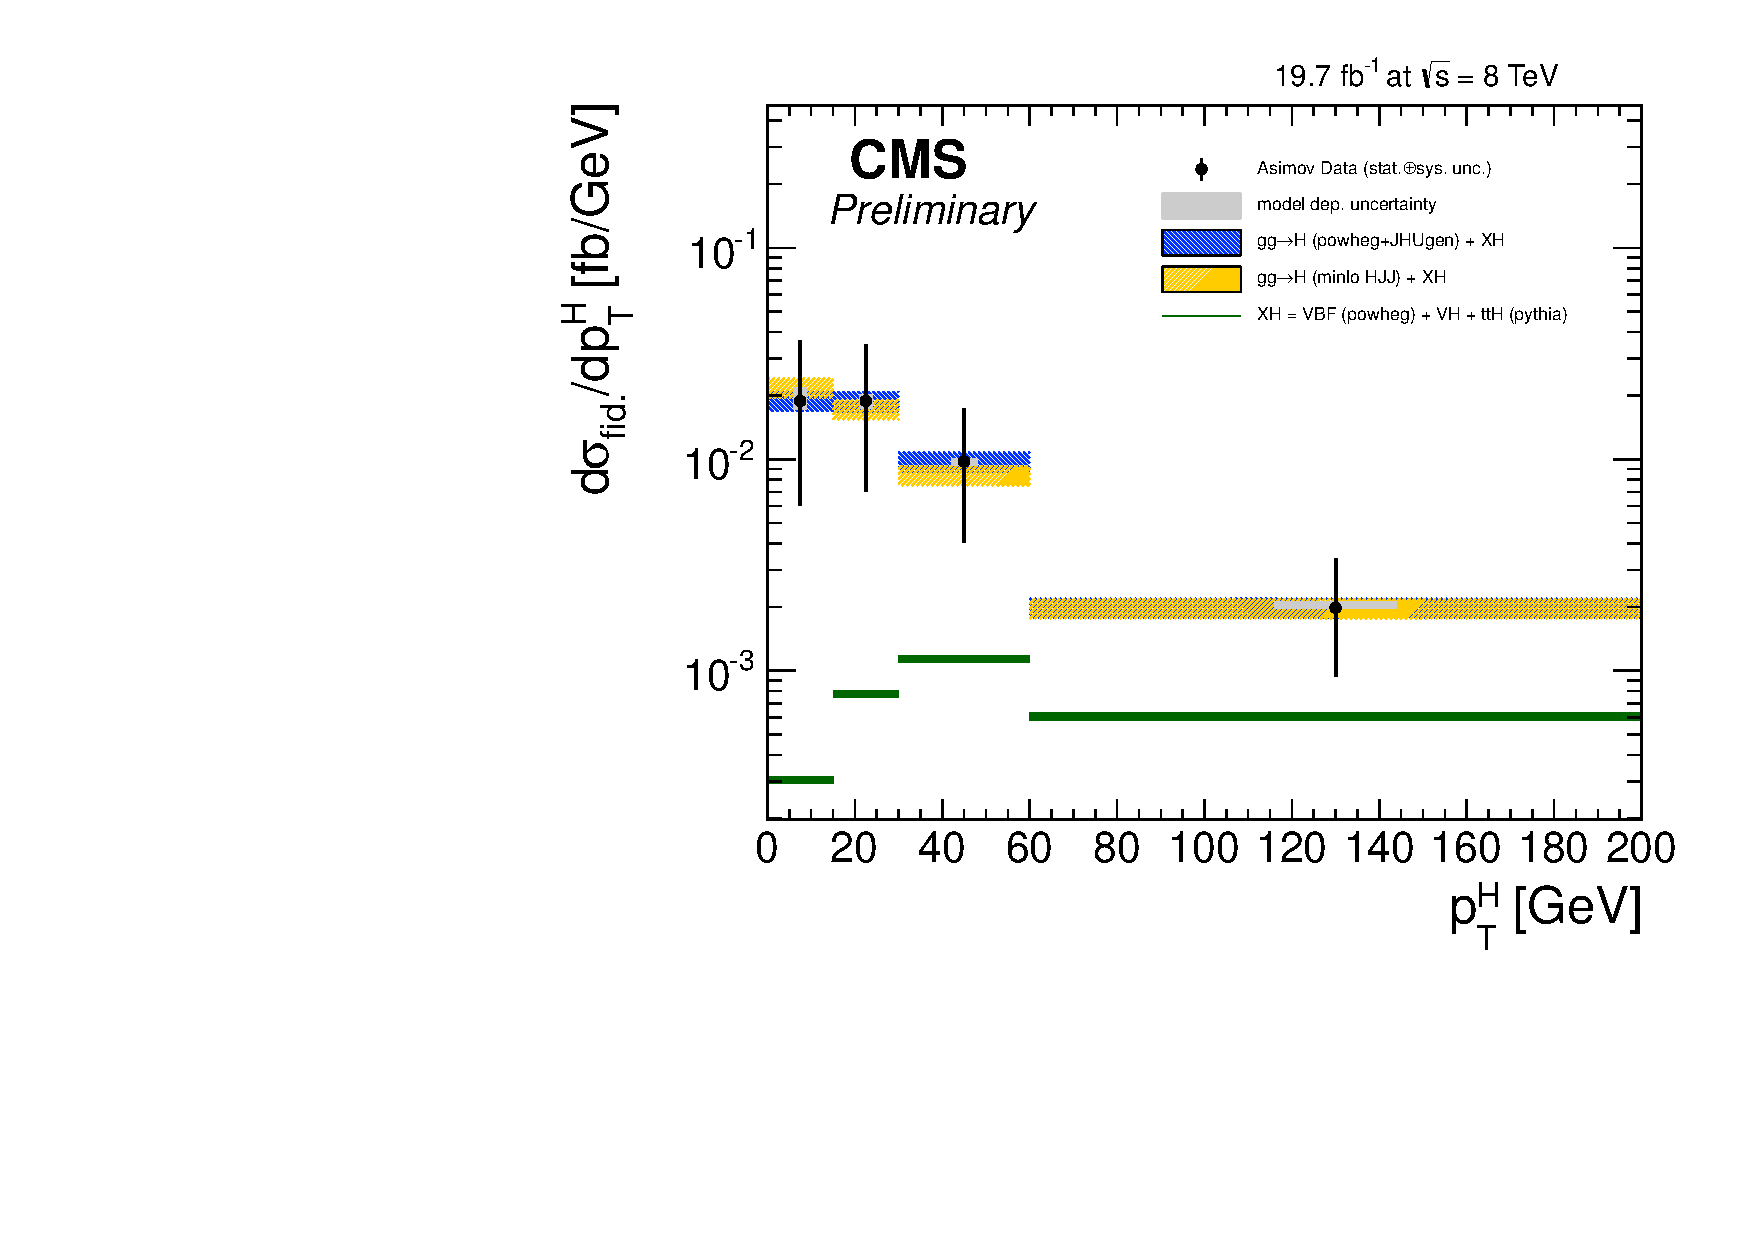
\includegraphics[width=0.48\textwidth,angle=0]{Plots/pT4l_unfoldwith_SM_125_logscale.pdf}
%      \label{fig:differential-results-fixfrac:a}
%    }
%    \subfigure[$\mathrm{m}(\mathrm{Z}_{2})$]{
%      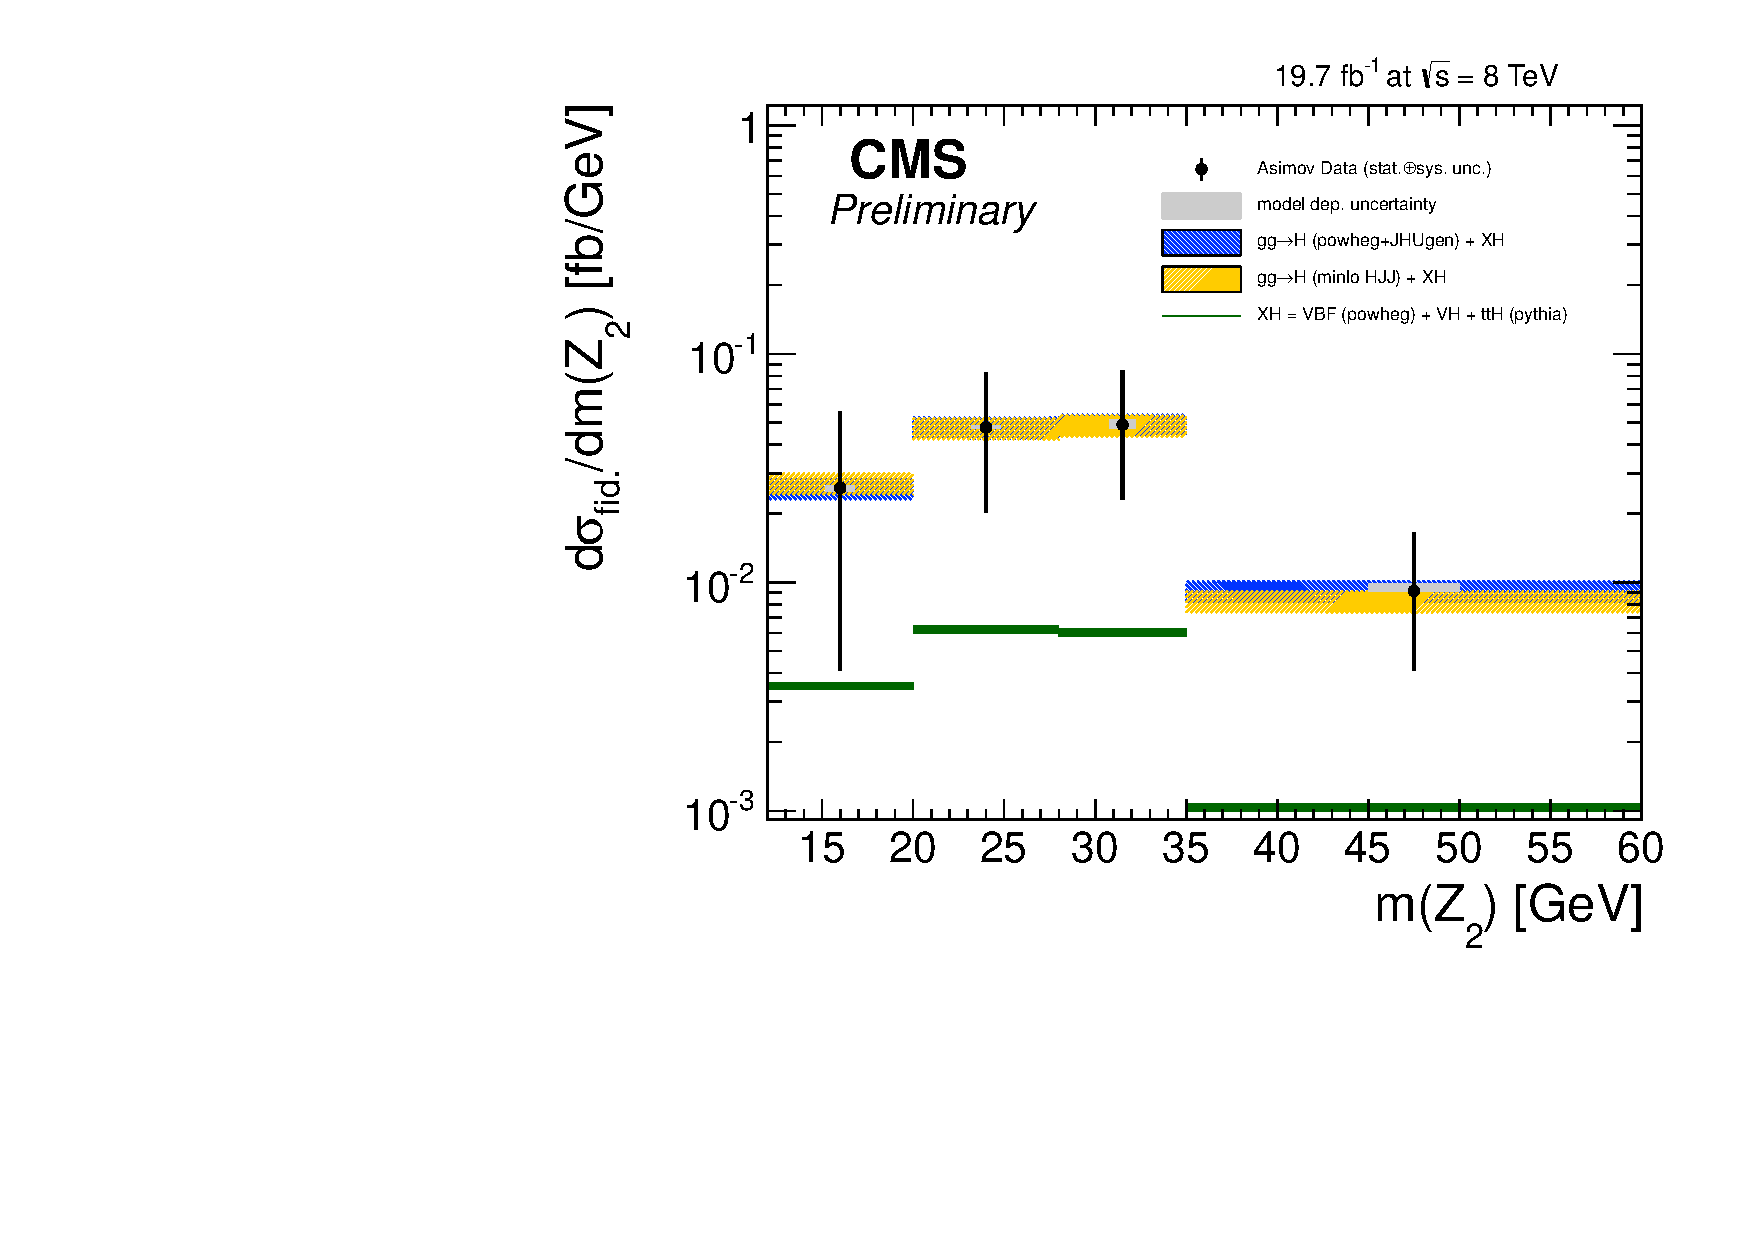
\includegraphics[width=0.48\textwidth,angle=0]{Plots/massZ2_unfoldwith_SM_125_logscale.pdf}
%      \label{fig:differential-results-fixfrac:b}
%    } \\
%    \subfigure[$|y(\mathrm{H})|$]{
%      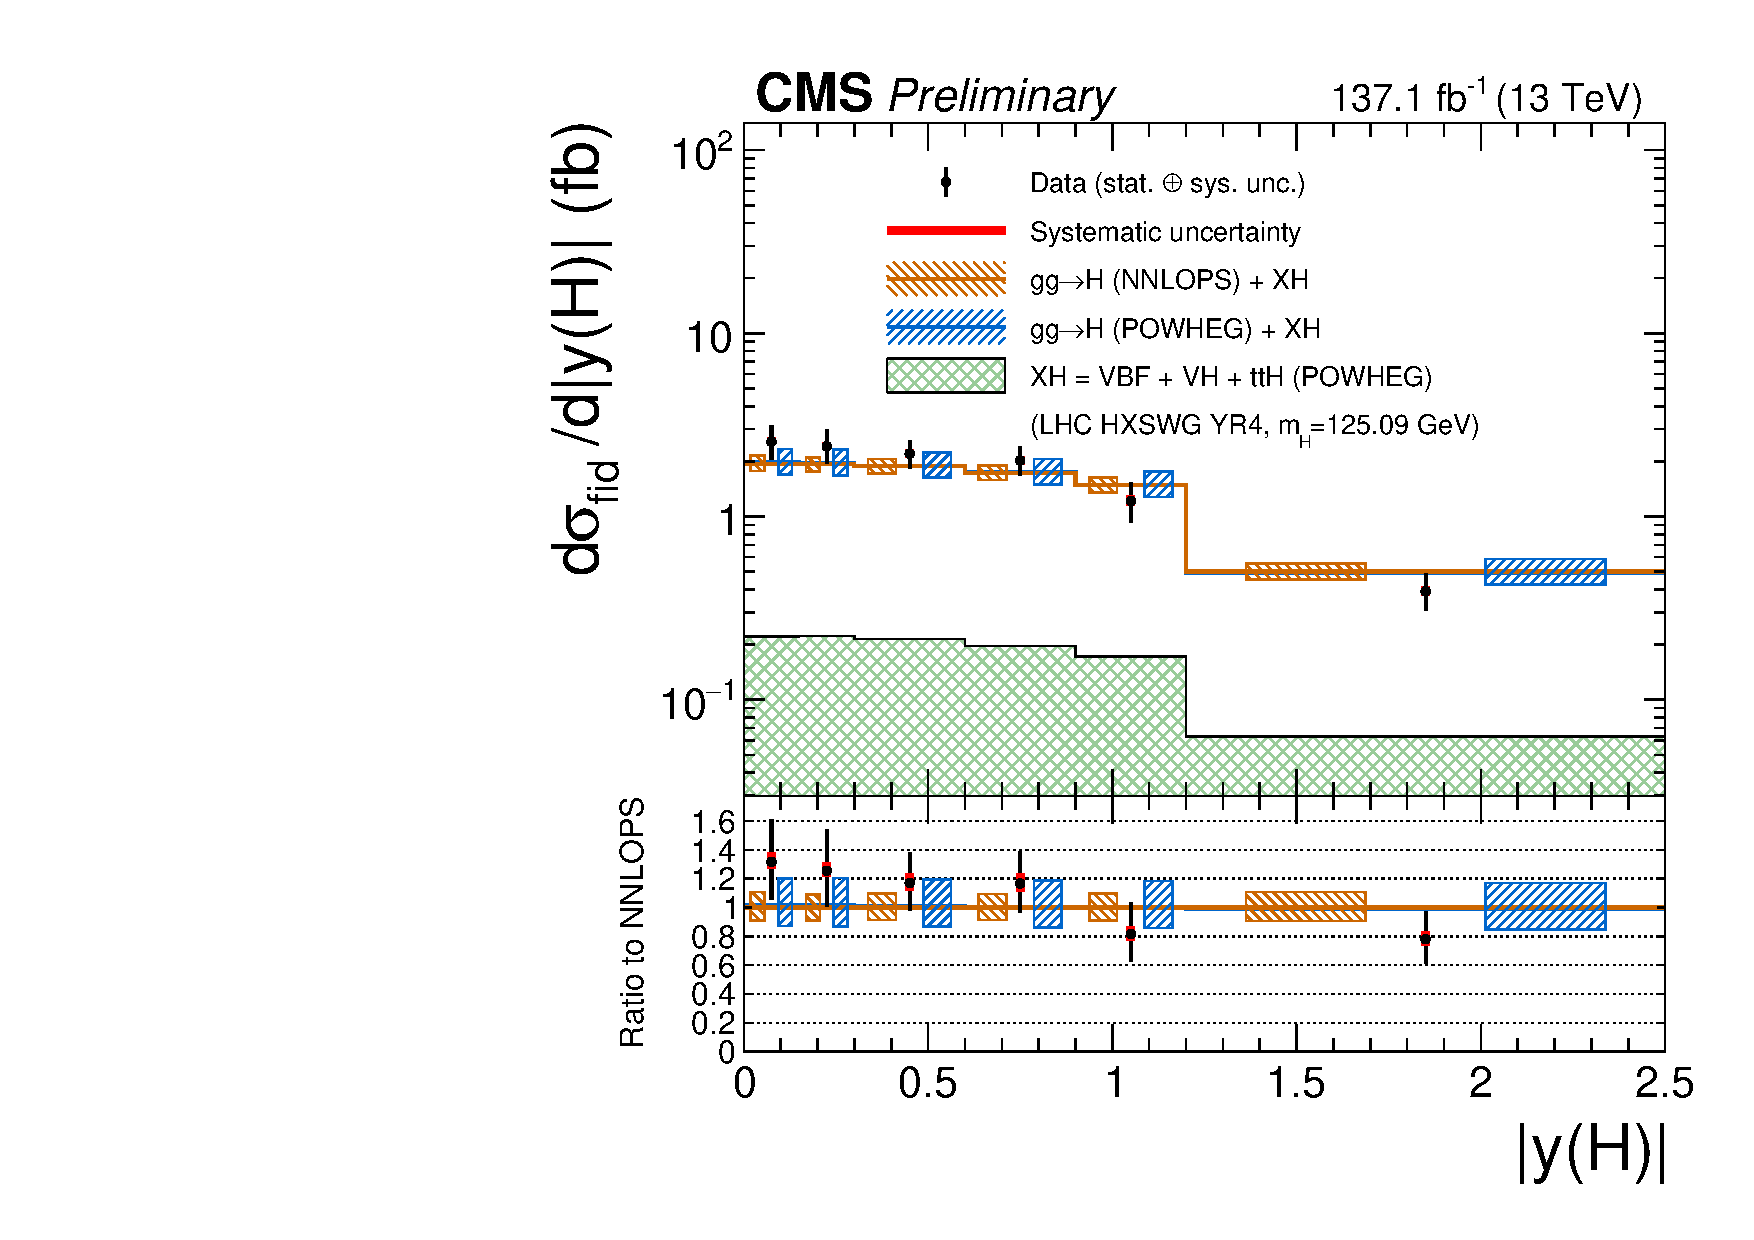
\includegraphics[width=0.48\textwidth,angle=0]{Plots/rapidity4l_unfoldwith_SM_125_logscale.pdf}
%      \label{fig:differential-results-fixfrac:b}
%    }
%    \subfigure[$|\cos \theta^{*}|$]{
%      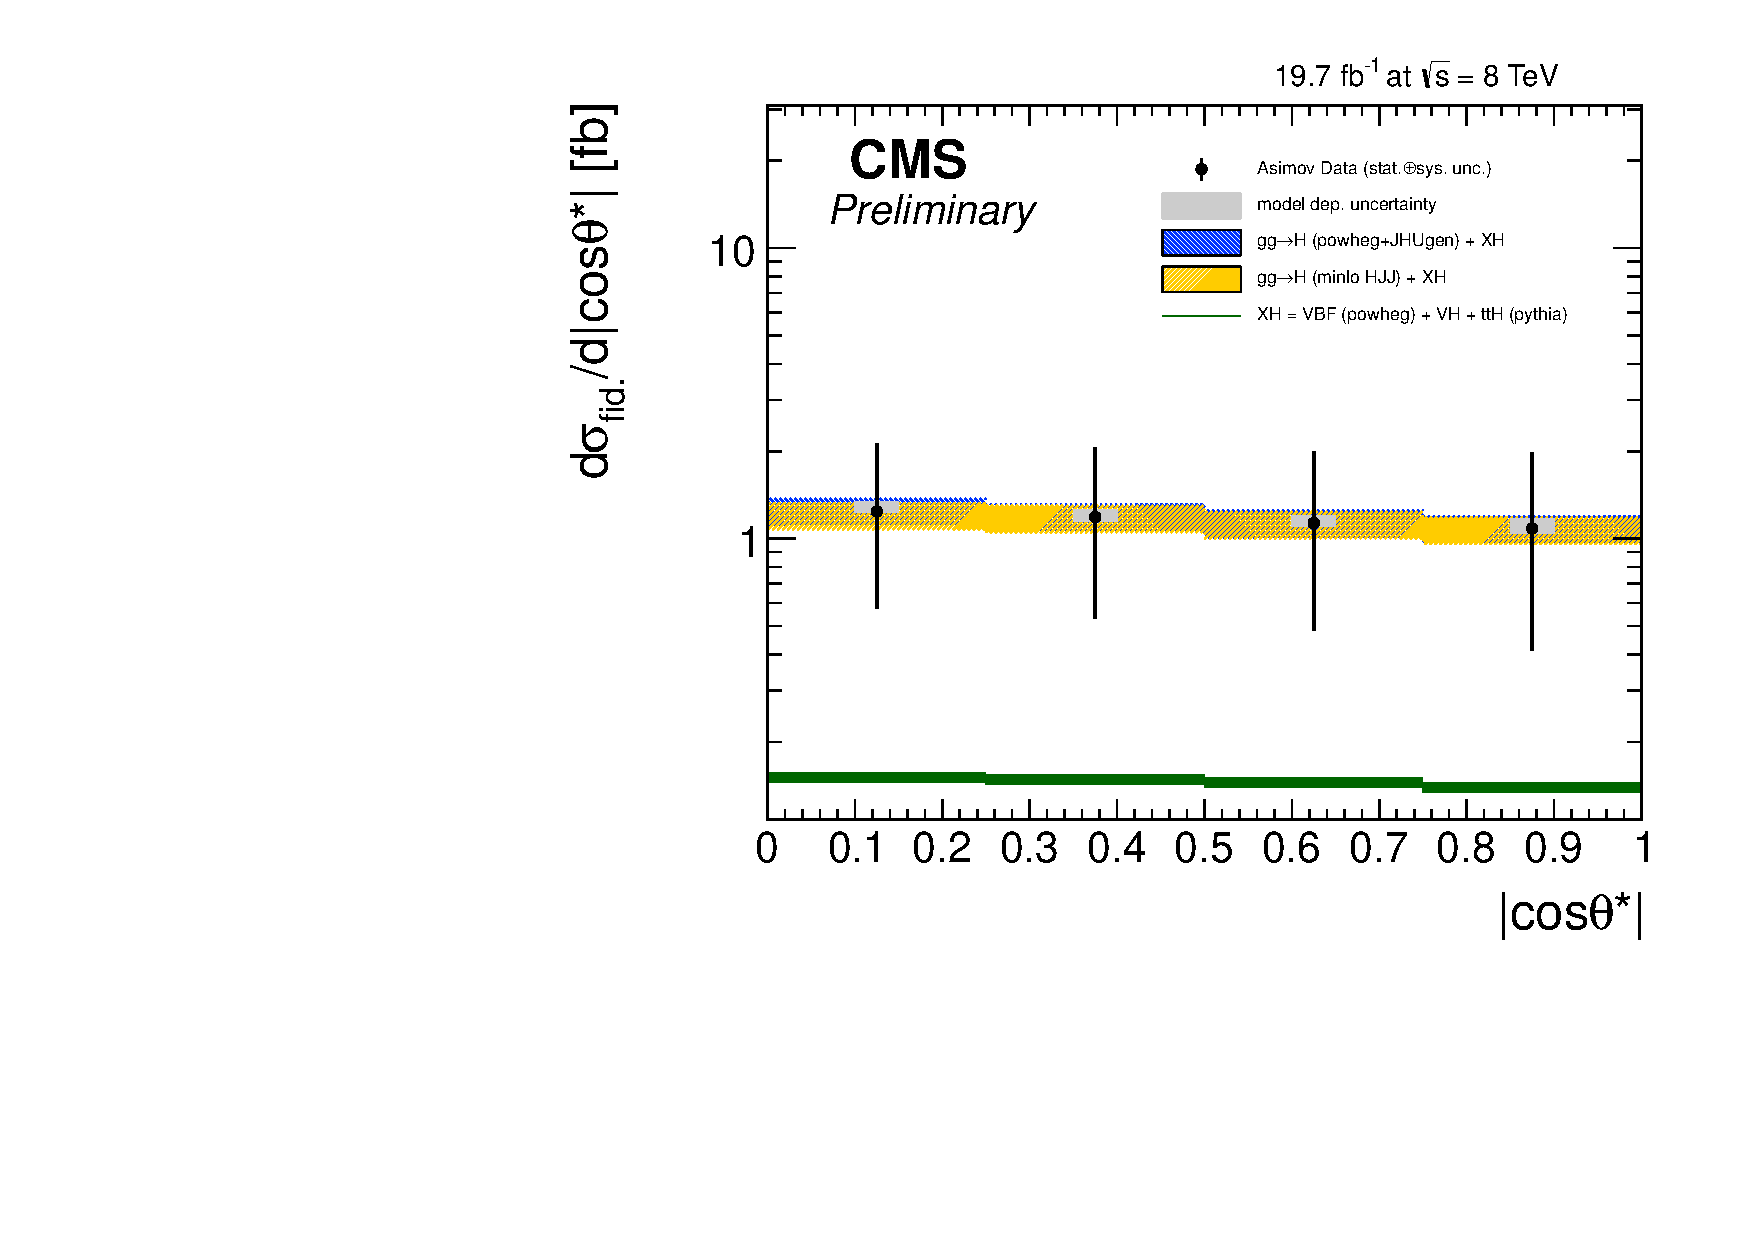
\includegraphics[width=0.48\textwidth,angle=0]{Plots/cosThetaStar_unfoldwith_SM_125_logscale.pdf}
%      \label{fig:differential-results-fixfrac:c}
%    } \\
%    \subfigure[N(jets)]{
%      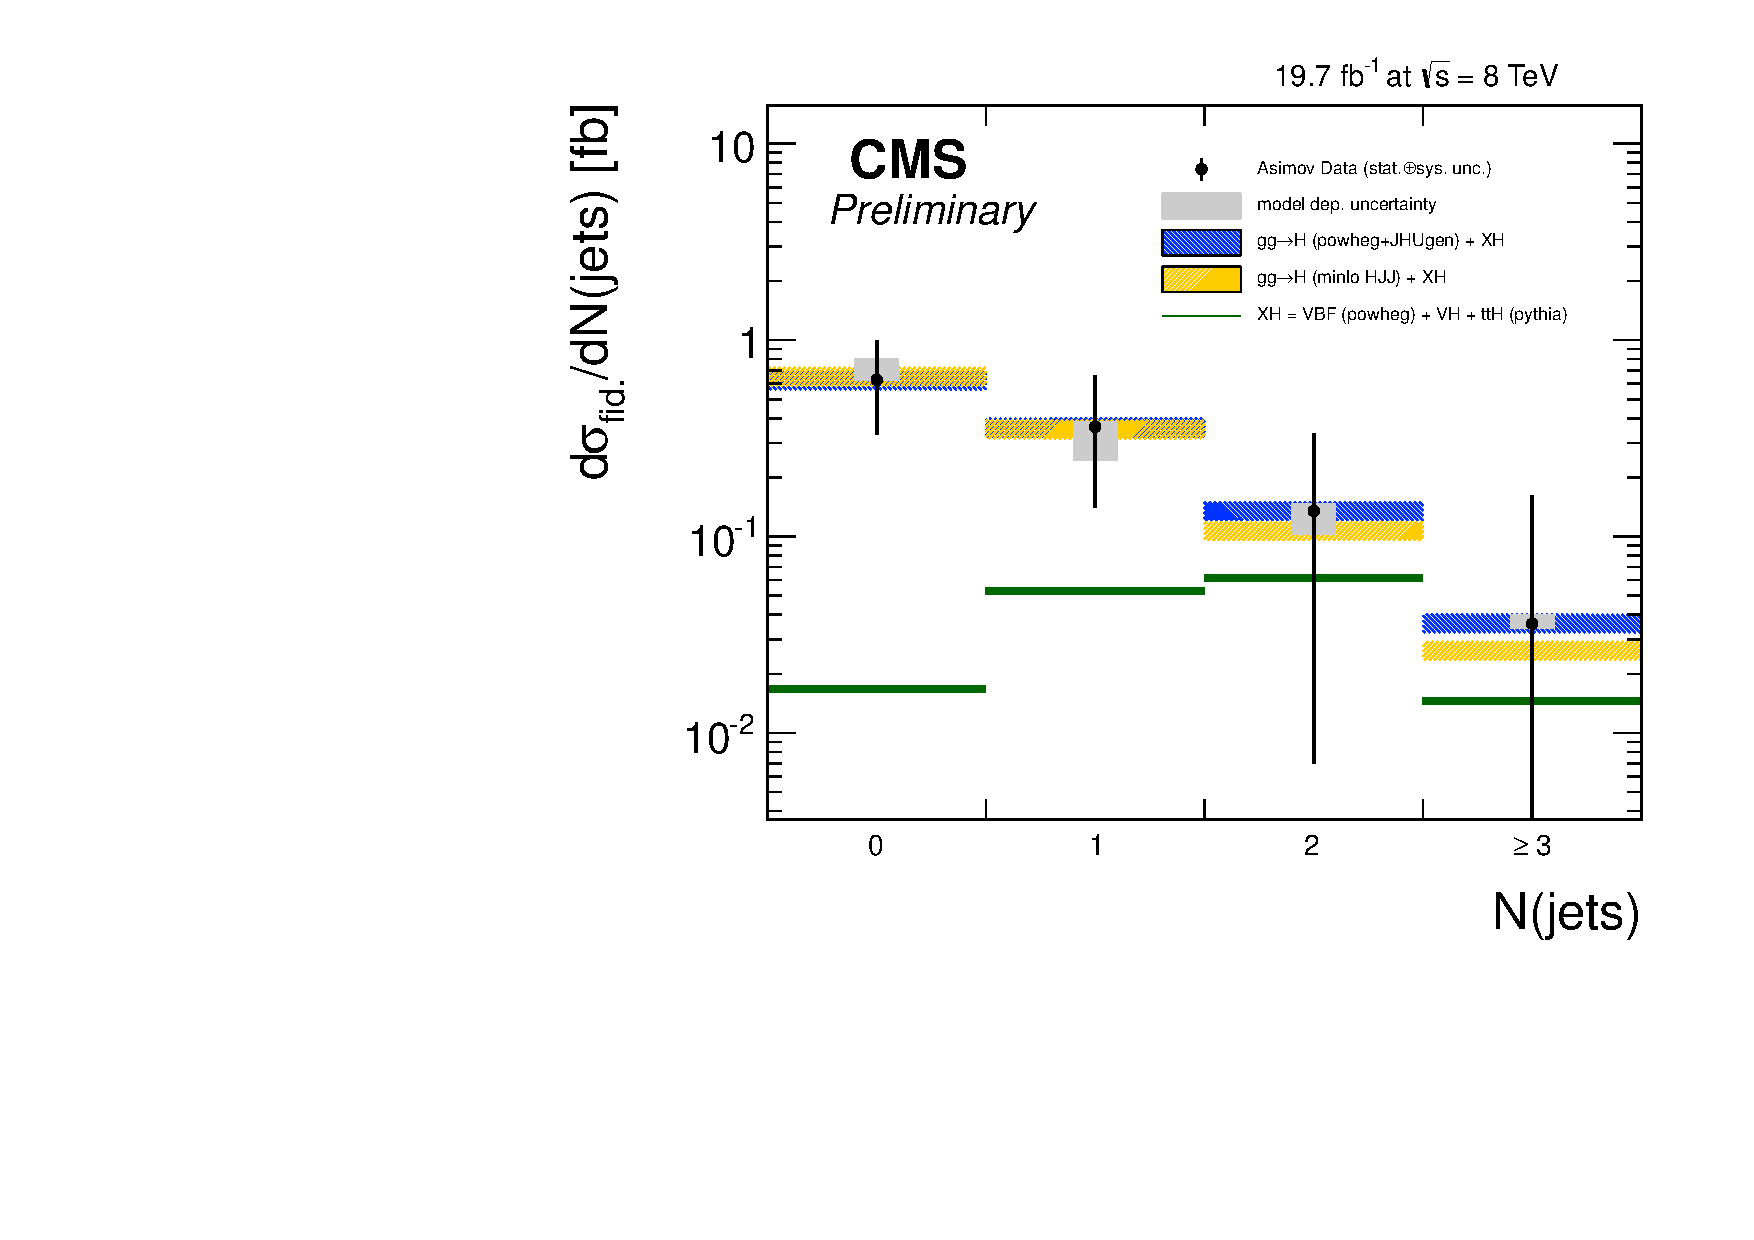
\includegraphics[width=0.48\textwidth,angle=0]{Plots/njets_reco_pt30_eta4p7_unfoldwith_SM_125_logscale.pdf}
%      \label{fig:differential-results-fixfrac:d}
%    }
%    \caption{Results of the differential cross section measurement for different observables. The predictions from {\sc powheg+JHUgen} and {\sc minloHJJ} are shown in blue and yellow, respectively. The central value of the measurement is obtained using the efficiencies from the {\sc powheg+JHUgen} gg$\rightarrow$H model with m(H)= 125 $\GeV$, and the error bar represents the combined statistical and systematic uncertainty. The grey box represents the additional uncertainty incurred when using different models to unfold the observed data distribution back to particle level. In this case, this model-dependance uncertainty is assessed by taking into account the experimental constraints from the exiting CMS measurements, as discussed in Section~\ref{sec:totalZZXSecSyst}. The fraction of $4e,4\mu$ and $2e2\mu$ in each bin are fixed to their SM expectations.
%    }
%  \label{fig:differential-results-restrictive_md}
% \end{center}
%\end{figure}


%\begin{landscape}
\begin{table}[htbp]
      \caption{
Results for individual channels of inclusive fiducial cross section of Z$\rightarrow 4l$ in mass window 50 to 105 GeV. \label{tab:z4l_results}
        }
\begin{tabular}{|c|c|c|c|c|}
\hline %---------------------------------------------------------
\hline %---------------------------------------------------------
\multicolumn{5}{|l|}{ Fiducial cross section Z$\rightarrow 4l$ (fb) } \\
\hline %---------------------------------------------------------
& 4l & $2e2\mu$ & $4\mu$ & $4e$ \\
\hline %---------------------------------------------------------
\vspace{-0.4cm} &&&&\\
Measured (stat.~$\oplus$~sys.)
&$4.813^{+0.700}_{-0.657}$
&$1.353^{+0.575}_{-1.177}$
&$2.413^{+0.595}_{-1.110}$
&$1.023^{+0.667}_{-1.023}$
\\
\vspace{-0.4cm} &&&&\\
\hline %---------------------------------------------------------
\vspace{-0.4cm} &&&&\\
\small {\sc powheg}
&$4.561^{+0.186}_{-0.190}$
&$1.570^{+0.064}_{-0.065}$
&$1.750^{+0.071}_{-0.073}$
&$1.241^{+0.051}_{-0.052}$
\\
\hline %---------------------------------------------------------
\end{tabular}
\end{table}
%\end{landscape}
%============



%============
%\begin{landscape}
\begin{table}[htbp]
      \caption{
Results for individual channels of inclusive fiducial cross section of H$\rightarrow 4l$ and the ratio between H$\rightarrow 4l$ and Z$\rightarrow 4l$, from a simultaneous fit of mass peaks of Z$\rightarrow 4l$ and H$\rightarrow 4l$ in mass window 50 to 140 GeV. \label{tab:incresults}
        }
\begin{tabular}{|c|c|c|c|c|}
\hline %---------------------------------------------------------
\hline %---------------------------------------------------------
\multicolumn{5}{|l|}{ Fiducial cross section H$\rightarrow 4l$ (fb) } \\
\hline %---------------------------------------------------------
& 4l & $2e2\mu$ & $4\mu$ & $4e$ \\
\hline %---------------------------------------------------------
\vspace{-0.4cm} &&&&\\
Measured (stat.~$\oplus$~sys.)
&$1.063^{+0.403}_{-0.269}$
&$0.468^{+0.273}_{-0.206}$
&$0.250^{+0.169}_{-0.125}$
&$0.342^{+0.301}_{-0.204}$
\\
\vspace{-0.4cm} &&&&\\
\hline %---------------------------------------------------------
\vspace{-0.4cm} &&&&\\
\small gg$\rightarrow$H({\sc pohwheg+JHUgen}) + XH 
&$1.161^{+0.125}_{-0.125}$
&$0.540^{+0.058}_{-0.058}$
&$0.326^{+0.035}_{-0.035}$
&$0.295^{+0.032}_{-0.032}$
\\
\vspace{-0.4cm} &&&&\\
\hline %---------------------------------------------------------
\vspace{-0.4cm} &&&&\\
\small gg$\rightarrow$H({\sc minloHJJ}) + XH 
&$1.143^{+0.123}_{-0.123}$
&$0.540^{+0.058}_{-0.058}$
&$0.317^{+0.034}_{-0.034}$
&$0.285^{+0.031}_{-0.031}$
\\
\hline %---------------------------------------------------------
\hline %---------------------------------------------------------
\multicolumn{5}{|l|}{ Ratio of fiducial cross sections H$\rightarrow 4l$ / Z$\rightarrow 4l$ } \\
\hline
& 4l & $2e2\mu$ & $4\mu$ & $4e$ \\
\hline %---------------------------------------------------------
\vspace{-0.4cm} &&&&\\
Measured (stat.~$\oplus$~sys.)
&$0.213^{+0.091}_{-0.071}$
&$0.325^{+0.226}_{-0.152}$
&$0.105^{+0.076}_{-0.053}$
&$0.297^{+0.317}_{-0.181}$
\\
\vspace{-0.4cm} &&&&\\
\hline %---------------------------------------------------------
\vspace{-0.4cm} &&&&\\
\small gg$\rightarrow$H({\sc pohwheg+JHUgen}) + XH %and Z$\rightarrow 4l$ ({\sc powheg}) 
&$0.254^{+0.040}_{-0.036}$
&$0.344^{+0.054}_{-0.049}$
&$0.185^{+0.029}_{-0.026}$
&$0.237^{+0.037}_{-0.034}$
\\
\hline %---------------------------------------------------------
\vspace{-0.4cm} &&&&\\
\small gg$\rightarrow$H({\sc minloHJJ}) + XH %and Z$\rightarrow 4l$ ({\sc powheg}) 
&$0.250^{+0.039}_{-0.036}$
&$0.344^{+0.054}_{-0.049}$
&$0.180^{+0.028}_{-0.026}$
&$0.230^{+0.036}_{-0.033}$
 \\
\hline %---------------------------------------------------------
\hline %---------------------------------------------------------
\multicolumn{5}{|l|}{ Predicted fiducial cross section of Z$\rightarrow 4l$ (fb)} \\
\hline
& 4l & $2e2\mu$ & $4\mu$ & $4e$ \\
\hline %---------------------------------------------------------
\vspace{-0.4cm} &&&&\\
\small {\sc powheg} 
&$4.578^{+0.186}_{-0.191}$
&$1.571^{+0.064}_{-0.066}$
&$1.766^{+0.072}_{-0.074}$
&$1.241^{+0.051}_{-0.052}$
\\
\hline %---------------------------------------------------------
\end{tabular}
\end{table}
%\end{landscape}
%============


%============
%============
